% -------------------------------------------------------------
% -------------------------------------------------------------
\section{Introduction}
% -------------------------------------------------------------
\subsection{Work objectives}
Why is ITER so large? How have been determined its main dimensions? Are these dimensions sufficient to reach its scientific goals,  i.e. produce 500 MW of fusion power for pulses of 400s with a power amplification ratio of 10\footnote{\url{https://www.iter.org/sci/Goals}}? And what should be the size of tokamak fusion reactor: smaller or larger than ITER? How much additional power is required to reach positive power amplification? How does it affect the magnets and the plasma facing components? 

Answering these questions is the main motivation for this group work. During the few days dedicated to this work, you will have to answers some of these questions by working in small groups. Interactions between groups is highly encouraged: no one can be expert of all the various physical and technological fields required to build a fusion machine, so group work is essential. When necessary, results will be shared between groups.

In the first part of the work, you will derive from a 0-dimensional approach the necessary equations to deduce a couple $(R_0, B_0)$ for a given reactor project of prescribed $(P_{DT}, Q)$. By proceeding this way, some other characteristics of the plasma (namely the shape of the plasma, including elongation and aspect ratio, the average ion mass $\hat M$, the edge safety factor $q_a$ and the density $n_N$ normalised to the Greenwald density $n_G$) will have to be prescribed by other considerations. This method will be applied to deduce the ITER parameters $(R_0, B_0)$. 

Each group results will be presented and shared with each others during the Part 1 evaluation. Once done, you will have to fix the main dimensions of the tokamak to be build. In the Part 2, groups will then focus on particular aspects of the machine: magnets, MHD stability, plasma facing components, safety and remote handling, external heating systems, etc. In case of problems, questions or design change requests, groups will be able to exchange between each other, or even to organise a general meeting in which topics affecting all groups can be discussed.

% -------------------------------------------------------------
\subsection{Schedule (2019)}
\begin{itemize}
\item Thursday and Friday 7 and 8th of March: Part 1
\item Monday 11th of March: groups restitution
\item From Tuesday 12th to Thursday 14th: Part 2
\item Friday 15th of March: Final groups restitution
\end{itemize}

% -------------------------------------------------------------
% -------------------------------------------------------------
\section{Part 1: Derivation of the Governing Relations}
The objective of this work is to deduce the main dimensioning parameters of a tokamak machine, namely the large radius $R_0$ and the magnitude of the (toroidal) magnetic field $B_0$ (on-axis, i.e. at normalised radius $\rho=0$) for a given couple of fusion power $P_{fus}$ and amplification factor $Q$. Since we are seeking two parameters, we will try to develop a 0D-approach sufficient to get two independent equations starting from the definition of $P_{fus}$ and $Q$. 

% --------------------------------------------
\subsection{Preamble on Units}
The International System of Units (SI) should be used. Quantities which are \emph{not} expressed in SI units should be emphasised with a specific symbol, for example with hats ``$\hat{...}$''. When possible, try to combine all numerical values (coming from physical constants) into a single constant $C$. In a later stage, these equations will be rewritten in a convenient set of units commonly used in tokamak physics.


% --------------------------------------------------
\subsection{Reminder: plasma geometry}



The usual plasma equilibrium are illustrated in figure \ref{fig:tokamakequilibrium_parameters}. If $\theta$ is the poloidal angle ($\theta=0$ on the equatorial plane), then one has the following relationships\footnote{The circular plasma corresponds to the limit case $\kappa=1$, $\delta=0$. }:
\begin{align}
	R =& R_0 + a \cos \left(\theta - \delta \sin\theta \right) \\
	Z =& \kappa a \sin \theta
\end{align}
The ITER case corresponds to $R_0=6.2$ m, $a=2$ m, $\kappa=1.85$, $\delta=0.5$. 

\begin{figure}
	\centering
	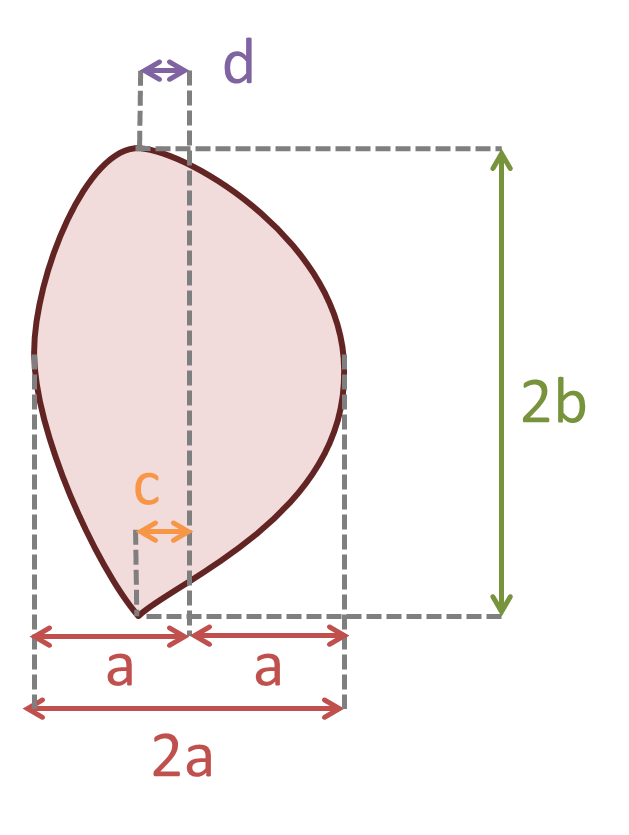
\includegraphics[width=0.39\linewidth]{figures/Tokamak_equilibrium1}
	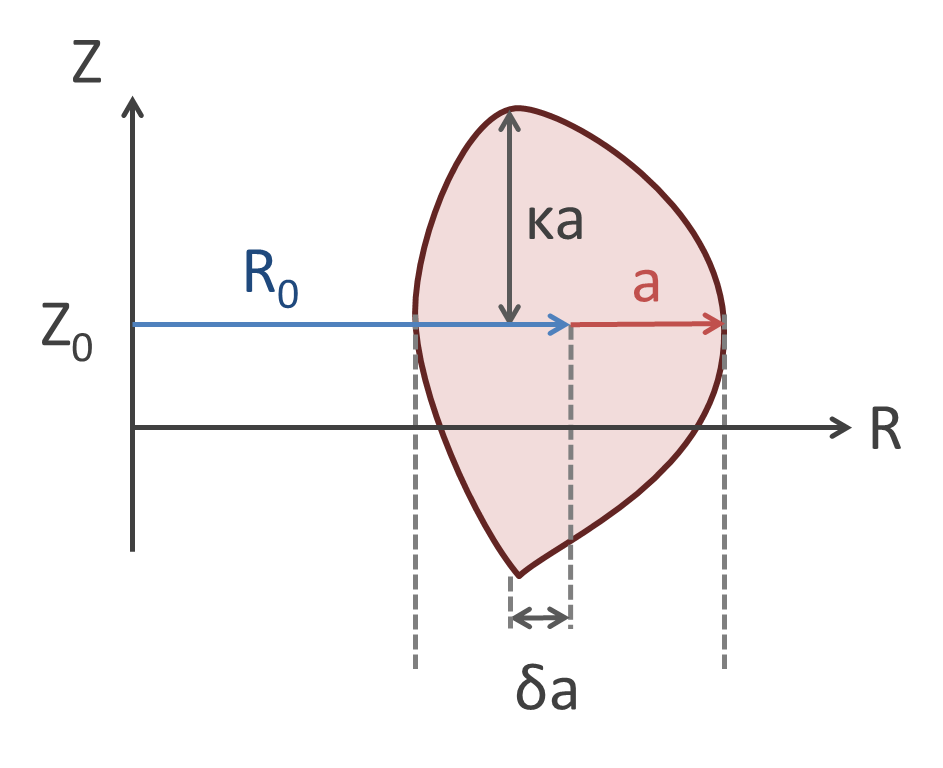
\includegraphics[width=0.59\linewidth]{figures/Tokamak_equilibrium2}
	\caption{Usual plasma equilibrium geometrical parameters. Plasma elongation: $\kappa=b/a$. Plasma triangularity: $\delta=\frac{c+d}{2a}$. }
	\label{fig:tokamakequilibrium_parameters}
\end{figure}



The volume of an elliptic tore can be approximated by:

\begin{equation}
V_t = 2\pi^2 \kappa R a^2
\end{equation}

\noindent
with $a$ the minor radius and $R$ the major radius of the tore. Here, $\kappa=b/a$ stands for the elongation of the plasma, $b$ being the largest radius of the ellipsoid (cf figure \ref{fig:tokamakequilibrium_parameters}). $\kappa=1$ for a circular cross-section, and is larger than unity for an elongated plasma.


Introducing the inverse aspect ratio $\varepsilon$ defined as $\varepsilon  \doteq a /R$, the volume then reads:

\begin{equation}
\boxed{
	V_t = C_V \varepsilon^2 R^3
}
\label{eq:tore_volume}
\end{equation}
\noindent
with $C_V = 2\pi^2$ and $\kappa=1$\footnote{Later eventually, $\kappa$ could be varied through the constant $C_V$ }. 


% --------------------------------------------
\subsection{Fusion Power $P_{fus}$}
\subsubsection{Fusion reactivity}
To get nuclear fusion, nuclei have to come close enough to each other. Nuclear forces can overcome their mutual electrostatic repulsion provided their distance becomes sufficiently close, in the order of 1 Fermi ($10^{-15}$m). %This would require temperatures of the order of 720 keV for head-on collisions of thermal particles to lead to fusion reactions in a classical way. Actually, quantum physics has to be taken into account in the process. 

However, both in tokamaks and in stars interiors, fusion reactions take place predominantly due to the tunnel effect. Crossing this barrier can be quantified in a probabilistic manner with the reaction rate $R$ $[\mathrm{reaction/m^3 s}]$, defined as the probability of reaction per unit time and volume. 

The reaction rate between mono-energetic ions of density $n_1$ $\mathrm{[m^{-3}]}$ striking target ions of density $n_2$ $\mathrm{[m^{-3}]}$ is proportional to the effective cross-section\footnote{The cross-section is expressed as a surface quantity and measures the probability of a reaction from a single nucleus target.} area $\sigma$ $\mathrm{[m^2]}$ and to the velocity difference $v_{12}$ between the two species:

\begin{equation*}
r_{12} = n_1 n_2 \; \sigma v_{12}
\end{equation*}

The quantity $\sigma v_{12}$, which depends on the kinetic energy of the colliding particles, is called the reactivity ($\mathrm{[m^3/s]}$). Note that the reaction rate $r_{12}$ is proportional to the square of the density of the mixture. 

In fusion plasmas, ions are not mono-energetic. They are assumed to have Maxwellian velocity distributions. The average reactivity $\langle \sigma v \rangle_{12}$ derives from the following expression:

\begin{equation*}
\left < \sigma v \right >_{12} 
= \int_{-\infty}^{+\infty} \int_{-\infty}^{+\infty} 
\sigma(v_{12}) v_{12}\;  f_1(v_1) f_2(v_2) \; dv_1dv_2
\end{equation*}

Finally, the average reaction rate $R_{12}$ reads:

\begin{equation*}
R_{12} = n_1 n_2 \; \left < \sigma v \right >_{12}
\end{equation*}

It governs the time evolution of both densities: $dn_1/dt = dn_2/dt = -R_{12}$.


The reactivity depends of the temperature and its evolution is known from the measurements of the cross-sections. The temperature dependence of the reactivity $\langle \sigma v \rangle_{12}$ is plotted on figure \ref{fig:reactivity} for several fusion reactions (interpolated data from \cite{Huba2013}). 

\begin{figure} 
    \begin{center}
        %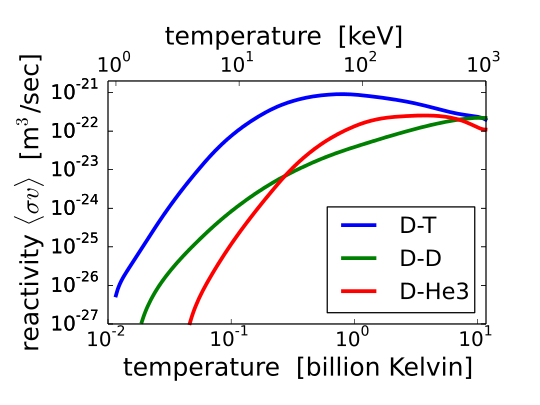
\includegraphics[width=0.75\textwidth]{figures/reactivity_DT.png}
        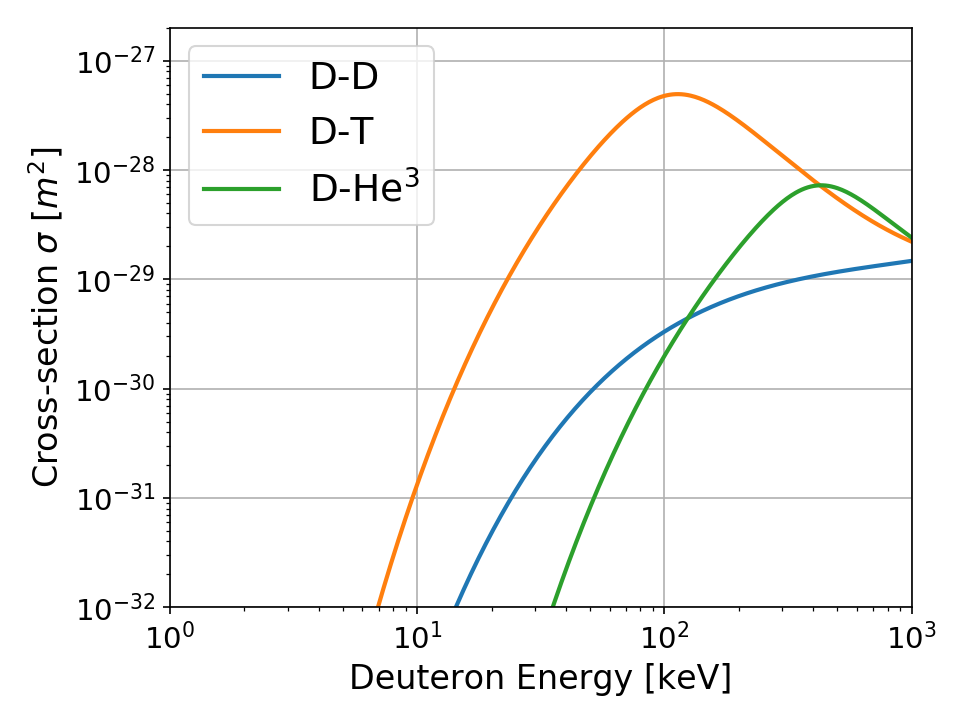
\includegraphics[width=0.49\textwidth]{figures/Fusion_cross-section.png}
        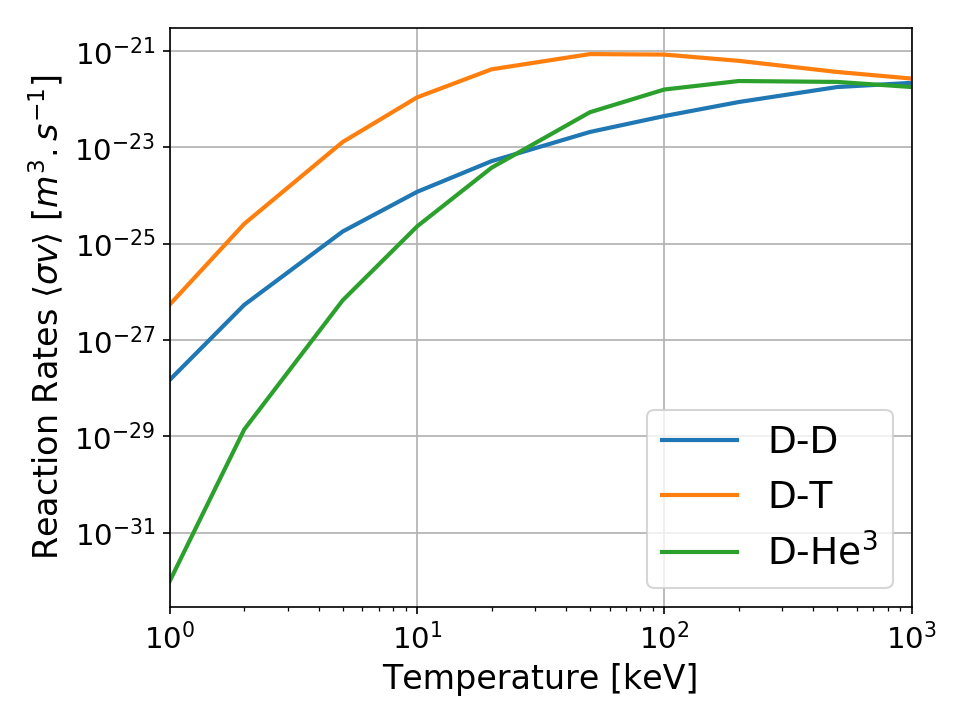
\includegraphics[width=0.49\textwidth]{figures/Fusion_Reactivity.png}
        \caption{Fusion reactions cross-sections (left) and reactivity (right), data taken from \cite{Huba2013} }
        \label{fig:reactivity_adv}
    \end{center}
\end{figure}

Of course, there is interest in operating a fusion reactor at the lowest temperatures. Looking to the figure \ref{fig:reactivity}, the mixture D-T seems the "easiest" way to initiate fusion reactions, since the D-T reaction  has the maximum reactivity at lowest temperature of all fusion reactions. The D-T reactivity reaches its maximum for a temperature of 64 keV, corresponding to a temperature of $742\,10^6$ K. The D-T reaction is \cite{FusionCEA1987}: 

\begin{equation*}
    \mathrm{D + T} \longrightarrow \mathrm{{}^4 He~(3.56~MeV) + n~(14.03~MeV)}
\end{equation*}

The D-T reaction leads to a total released energy of $E_{DT}$ = 17.59 \si{MeV} = $2.82\times 10^{-12} \si{J}$ per fusion reaction\footnote{This value can be compared to the 200 MeV released by $^{235}$U fission. Yet, the energy release \emph{per nucleon} ($i.e.$ per kilogram) is approximately 4 times larger for fusion than for fission reactions.}. Notice that the ratio of the total energy to that carried by the alpha particles $\lambda \doteq 17.59/3.56 \approx 4.94$ is not exactly equal to 5 as one would expect on the basis of momentum conservation. Actually, this ratio \emph{is obviously} consistent with momentum conservation, as it should, provided one takes into account relativistic effects. This point is detailed in section \ref{appendix:fusion_power}.

The fusion power per unit volume $p_{DT}$ produced by the fusion of the nuclei of deuterium and tritium reads: 
\begin{equation*}
  p_{DT} = n_D n_T \left< \sigma v \right>_{DT} E_{DT}
\end{equation*}
with $n_D$ and $n_T$ the deuterium and tritium density and $\left< \sigma v \right>_{DT}$ the D-T reactivity. Assuming equal deuterium and tritium densities:
\begin{equation*}
  n_D = n_T = \frac{n}{2}
\end{equation*}
with $n$ the electron density, then the thermonuclear power density is:
\begin{equation*}
  p_{DT} = \frac{1}{4} n^2 \left< \sigma v \right>_{DT} E_{DT}
\end{equation*}

Assuming a constant reactivity in the plasma ("flat profile hypothesis") and using the tore volume $V$, the fusion power is: 
\begin{equation}
  P_{fus} = \frac{V}{4}
    n^2 \left< \sigma v \right>_{DT} E_{DT}
\end{equation}

% --------------------------------------------------
\subsubsection{Relationship 1}
Using the tore volume eq.\ref{eq:tore_volume}, one readily obtains the fusion power:

\begin{equation}
\boxed{
	P_{fus} = \frac{C_V}{4}
  				\varepsilon^2 R^3
				n^2 \left< \sigma v \right>_{DT} E_{DT}
	}
	\label{eq:FusionPower1}
\end{equation}

This is the first equation relating $P_{fus}$ to the geometrical parameter $R$. However, it is not usable yet, since from figure \ref{fig:reactivity}, the reactivity $\left< \sigma v \right>$ clearly depends of the temperature. It will be thus necessary for the following to define the temperature at which the machine should operate. This will be part of the physical constraints discussion in the next section. 


This total fusion power is distributed among the alpha particles and the neutrons: 
\begin{equation}
	P_{fus} 
	= 
	P_\alpha + P_n 
	= 
	\lambda \; P_\alpha
\label{eq:P_fus_Palpha}
\end{equation}
where we recall that $\lambda \approx 4.94$. Due to the mass ratio, almost 80\% of the power is carried by the neutrons. 

% --------------------------------------------------
% --------------------------------------------------
\subsection{Amplification factor $Q$}


% -------------------------------------------------------
\subsubsection{Definition of $Q$}
Let's start from definition of the plasma amplification factor. The amplification factor is defined as the ratio of the fusion power $P_{fus}$ to the external heating power supplied $P_{ext}$\cite[p.12]{Wesson2004}, \cite[(3.4)]{FusionCEA1987}:

\begin{equation}
	Q \doteq \frac{P_{fus}}{P_{ext}}
\label{eq:definition_Q}
\end{equation}

Importantly, notice that $Q$ \emph{does not} encompass -- by far -- the entire question of the energetic efficiency of a fusion reactor. Indeed, in particular, it does neither account for the energy used for cryogenic purposes (as required by the use of superconductors) nor for the conversion factor of thermal to electric energy\footnote{This point is often misleading for the public and it is important to be factually correct. Misleading statements concerning fusion and ITER power and energy since decades have been highlighted in \url{http://news.newenergytimes.net/2017/10/06/the-iter-power-amplification-myth/}. This led directly ITER to update its public information web pages on the Q-factor (cf. \url{https://www.iter.org/newsline/-/2845}).  Cf. also the follow-up \url{http://news.newenergytimes.net/2017/12/11/evidence-of-the-iter-power-deception/}}.

% ------------------------------------------
\subsubsection{Power Balance: sources terms}
At equilibrium, sources terms equal sink terms:
\begin{equation}
	\sum_{sources} P = \sum_{loss} P
	\label{eq:power_balance_general}
\end{equation}
where the losses terms will be discussed in the next subsections.

To the contrary with neutrons which leave the plasma, charged $\alpha$ nuclei are confined by the magnetic field and should ideally transfer their energy to the main ions before being extracted\footnote{There are basically 2 ways for this energy transfer. Since the collision frequency scales like the velocity difference between the colliding species to the power $-3$ ($\nu_{coll,ss'}\sim n_{s'}/\Delta v_{ss'}^3$), alpha particles transfer their energy dominantly to the electrons, which are much faster due to their low inertia. Then two routes are possible for the energy transfer from the electrons to the ions. Either via collisions, or via turbulence. In the latter case, the mediator are the electrostatic plasma waves. The relative weight of those two channels is still a matter of research.}. The total -- or \emph{net} -- heating power $P_{net}$ is the sum of the auxiliary plasma heating,  $P_{ext}$, of Ohmic heating $P_\Omega$ and of alpha heating $P_\alpha$, minus the radiative losses $P_{rad}$\footnote{The reason why the radiative losses are included comes from the definition of the confinement time, described in a next section.}:

\begin{equation}
	P_{net} 
	\doteq 
	P_\alpha + P_\Omega + P_{ext} - P_{rad}
\label{eq:definition_net_power}
\end{equation}

In the following, we will assume that the ohmic contribution is negligible. Radiative losses are discussed in Appendix \ref{appendix:radiative_losses}. For the sake of simplicity, we will replace hereafter the radiative losses by the coefficient $0\leq \gamma_{rad} \leq1$:
\begin{equation*}
P_{net} \doteq \gamma_{rad} (P_\alpha + P_{ext})
\end{equation*}

Using \ref{eq:P_fus_Palpha} and \ref{eq:definition_Q}:
\begin{equation}
\boxed{
	P_{net} 
	\doteq 
	\gamma_{rad}
	P_{fus}
	\frac{1 + Q/\lambda}{Q}
}
\label{eq:Pnet_as_Pfus_Q}
\end{equation}
Replacing $P_{fus}$ by its expression eq.\ref{eq:FusionPower1}, one finally obtains:
\begin{equation}
\boxed{
	P_{net} 
	= 
	\gamma_{rad}
	\frac{C_V}{4}
	\varepsilon^2 R^3
	n^2 \left< \sigma v \right>_{DT} E_{DT}
	\frac{1+Q/\lambda}{Q}
 }
\label{eq:Pnet_QnTR_adv}
\end{equation}

Now that we have expressed the $P_{net}$ term from the equilibrium relation \ref{eq:power_balance_general}, one needs to express the loss terms.

% --------------------------------------------------
\subsubsection{Power Balance: Losses and Energy Confinement time $\tau_E$}

The losses origins being diverse, it is convenient to group all losses into one term $P_{loss}$\cite[p.9]{Wesson2004}:

\begin{equation}
	P_{loss} 
	\doteq 
	\frac{ W }{ \tau_E } 
\label{eq:definition_confinement_time_global}
\end{equation}
\noindent
where $W$ is the total thermal plasma energy and where we have defined $\tau_E$ as the energy confinement time. 

Usually, the energy confinement time $\tau_E$ is defined as the characteristic time at which this energy is lost from the plasma due to thermal transport (conduction and convection), either by collisional conduction or by turbulent thermal convection. This leads to the following (re)definition\cite[(3.2)]{FusionCEA1987}:
\begin{equation}
	P_{loss} 
	\doteq 
	P_{rad}
	+
	\frac{ W }{ \tau_E } 
\label{eq:definition_confinement_time}
\end{equation}
\noindent
which explains now why the radiative term has been put into the net power expression() \ref{eq:definition_net_power}). Note that this latter definition is consistent with the one used for the ITER scaling laws, discussed in the next sections.


% --------------------------------------------------
\subsubsection{Plasma Thermal Energy $W$}
The total internal energy of the plasma reads as follows:
\begin{equation*}
W  = \int \frac{3}{2} k_B \left( n_e T_e + n_i T_i \right ) dV 
\approx \int 3 n k_BT dV
\end{equation*}

\noindent
where the integral is performed over the plasma volume. Here, equal ion and electron temperatures have been assumed. Assuming flat density and temperature profiles and using the expression of the volume of a torus eq.\ref{eq:tore_volume}, the total plasma internal energy then reads:
\begin{equation}
W = 3 n k_B T V = 3 k_B C_V \varepsilon^2  n T R^3
\label{eq:total_energy_natural_units}
\end{equation}




% --------------------------------------------------
\subsubsection{Energy Confinement Time $\tau_E$}
Experimental results have shown that the energy time in ELMy H-mode tokamak plasmas (referred to as the ITER IPB98(y,2) scaling law \cite[eq.(20)]{ITERphysics_chap2}) is well represented -- the root means square error is about 15.6\% -- by the following scaling law:

\begin{equation}
	\tau_E = C_{SL} \hat M^{0.19} \kappa^{0.78} \varepsilon^{0.58} 
	\hat n^{0.41} \hat I_p^{0.93} R^{1.97} B^{0.15}  \hat P_{net}^{-0.69}
	\label{eq:scaling_law_IPB98(y,2)_adv}
\end{equation}

\noindent
with $C_{SL} = 0.0562$.


Here, $\hat I_p$ and $B$ are the plasma current and the toroidal magnetic field at the magnetic axis, respectively, $\hat n$ the line-averaged density, and $\hat M$ is the average ion mass (in Atomic Mass Unit)\footnote{Cf. also \url{http://fusionwiki.ciemat.es/wiki/Scaling_law}.}. 





% --------------------------------------------------
\subsubsection{Plasma Current $I_p$}

Integrating the Maxwell-Ampère equation over the whole plasma cross-section, and using Stokes' theorem, one gets:

\begin{equation*}
\int_\mathcal{S} (\nablabf\times \Bbf) \cdot \mathbf{dS} = 
\oint_\mathcal{C} \mathbf{B} \cdot \mathbf{d\ell}
= \mu_0 \int_\mathcal{S} \jbf \cdot \mathbf{dS} = \mu_0 I_p
\end{equation*}

Neglecting the elongation of the cross-section, the equation can be approximated as follows:
$$
2\pi a B_p = \mu_0 I_p
$$

\noindent
with $B_p$ the poloidal component of the magnetic field at the separatrix. In the limit of large aspect ratios, it can be easily related to the safety factor $q_a$ at the separatrix\footnote{Actually, $q_a$ is usually taken slightly inside the separatrix, at 95$\%$ of the poloidal magnetic flux.}:

\begin{equation*}
q_a \doteq \frac{a}{R} \frac{B_t}{B_p} 
\end{equation*}

\noindent
with $B_t$ the toroidal component of the magnetic field at the magnetic axis. Then it comes:

\begin{equation}
\boxed{\hat I_p = C_I \frac{\varepsilon^2}{q_a} \; R B}
\label{eq:plasma_current_adv}
\end{equation}

\noindent
where $\hat I_p$ is the current expressed in MA, and $C_I = 2\pi\, 10^{-6} /\mu_0 = 5$  ($\mu_0 = 4\pi\, 10^{-7} \si{H.m^{-1}}$).
Notice that $B_t$ has been safely replaced by $B$ since $B_p\ll B_t$ in tokamak plasmas. 

% --------------------------------------------------
\subsubsection{Power Balance: the link between $Q$ and $\tau_e$}
At equilibrium\footnote{Should the plasma not be at equilibrium and/or be subject to significant radiative losses in the confined region, then $P_{net}$ should be replaced by $(P_{net}-dW/dt-P_{rad})$. The subtraction of $P_{rad}$ ensures the balance equation to be consistent with the retained definition of $\tau_E$.}, i.e. from (eq.\ref{eq:power_balance_general}), one has:
\begin{equation}
	P_{net} = P_{loss}
\end{equation}

Using the expressions of $P_{net}$ (\ref{eq:Pnet_QnTR_adv}) and expending $P_{loss}$ (\ref{eq:definition_confinement_time}) using expressions of $W$ (\ref{eq:total_energy_adv}) and $\tau_E$ (\ref{eq:scaling_law_IPB98(y,2)_adv}) leads to
\footnote{Remind to include the parameter $\kappa^{0.78}$ which has been removed from the confinement time scaling law into the volume constant $C_V$ (as $\kappa^{-0.78}$)}:

\begin{equation}
	\left(
		\gamma_{rad} P_{fus} \frac{1 + Q/\lambda}{Q}
	\right)^{0.31}
	=
	C_{loss} C_V C_I^{-0.93} C_{SL}^{-1}
	M^{-0.19} \varepsilon^{-0.44}
  \hat n^{0.59} \hat T  q_a^{0.93} R^{0.1} B^{-1.08} 
\end{equation}

Which is the second equation relating the target $(P_{fus}, Q)$ to the machine parameters $(R,B)$. 

However, some unknowns still remain, for instance in the expression of the fusion power $P_{fus}$, which will be discussed in the next part.

% --------------------------------------------------
% --------------------------------------------------
% --------------------------------------------------
\section{Physical Constraints}
% --------------------------------------------------
% --------------------------------------------------
\subsection{Reactivity and Temperature range}
Without expanding the confinement time, equilibrium relationship (\ref{eq:power_balance_general}) can be written using (\ref{eq:Pnet_QnTR_adv}) and (\ref{eq:total_energy_adv}) simplifies into:
$$
n \tau_E 
=
C_{lawson}
\frac{Q}{1+Q/\lambda}
\frac{\hat T }{\left< \sigma v \right>_{DT} }
$$ 
with $C_{lawson} = 12\times10^3 e / (\gamma_{rad} E_{DT})\approx 6.818\times10^{-4}/\gamma_{rad}$ (width $E_DT$ in Joules). The latter expression is a form of the Lawson criteria, stating that the heating power should be higher than the thermal losses, ie.:
\begin{equation}
	n \tau_E 
	\geqslant
	C_{lawson}
	\frac{Q}{1+Q/\lambda}
	\frac{\hat T }{\left< \sigma v \right>_{DT} }
\label{eq:Lawson_criterium_temperature_adv}
\end{equation} 


The D-T fusion reactivity, as illustrated in figure \ref{fig:reactivity_adv}, depends of the temperature and peaks around $T \approx 66.5$ keV. Few empirical formulas or tabulations have been proposed, which can be found for instance the Bosch-Hale parametrization \cite[sec.9.8]{Hartwig2016} or the Brunelli \cite[sec.2.4]{FusionCEA1987}:
\begin{equation}
\left< \sigma v \right>_{DT} \approx 9.10^{-22}
\exp\left\{ -0.476 \left| \ln\frac{\hat T}{69} \right|^{2.25}\right\}
\;\;\;\textrm{m}^3.\textrm{s}^{-1}
\end{equation}
 
The value of $n \tau_E$ in (\ref{eq:Lawson_criterium_temperature_adv}) are illustrated in figure \ref{fig:ntau_E_vs_T_adv} using the above expression of the reactivity as a function of the temperature.

\begin{figure}[h]
	\begin{center}
	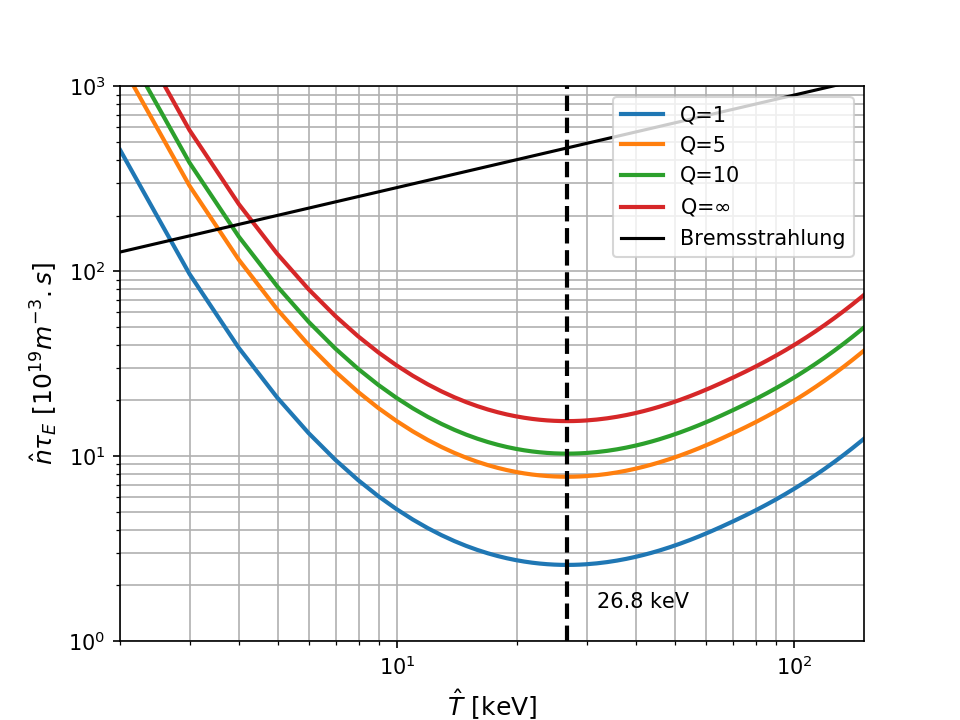
\includegraphics[width=0.9\textwidth]{figures/ntau_e_vs_T_loglog.png}
	\end{center}
    \caption{$\hat n \tau_E$ evaluated as a function of $\hat T$ and for different values of $Q$ ($\gamma_{rad}=1$). All curves have a minimum for $\hat T\approx 26.8$~keV. Break-even and ignition contours correspond to $Q=1$ and $Q \to\infty$ curves respectively.}
	\label{fig:ntau_E_vs_T_adv}
\end{figure}


It turns out that the product $\hat n \tau_E$ is minimum for a temperature $\hat T\approx 26.8$~keV, whatever the value of $Q$. Hence the optimal target temperature to consider for D-T reactions is around 26 keV. 


{\color{red}HERE ADD EXPLANATION FROM 26 to 15 keV}


In the temperature range $T_{\mathrm{[keV]}} \in [10.3-18.5]$ keV, it turns out that the reactivity $\left< \sigma v \right>_{DT}$ can well (with about 10$\%$ error) be approximated by \cite[(1.5.4)]{Wesson2004}: 

\begin{equation*}
\left< \sigma v \right>_{DT} 
\approx 
1.18\, 10^{-24}\; \hat T^2 \;\si{\left[m^3 s^{-1}\right]}
\end{equation*}




\ref{eq:FusionPower1}
\ref{eqn:beta_adv}

% --------------------------------------------------
% --------------------------------------------------
\subsection{Plasma Radiation}
In a fusion plasma, the three most important types of radiation are: 
\begin{itemize}
	\item Bremsstrahlung radiation, 
	\item line radiation (when the plasma contains impurity species), 
	\item synchrotron radiation.
\end{itemize}

Bremsstrahlung radiation is an important radiation loss in fusion plasma and usually dominates the two other radiation mechanisms for plasma temperature below then 20 keV. 

% ---------------------------------------------------------------------------
\subsection{Bremsstrahlung Radiation}
Bremsstrahlung radiation, i.e., "braking radiation" or "deceleration radiation", is the electromagnetic radiation produced by the deceleration of a charged particle when deflected by another charged particle (typically an electron by an atomic nucleus). The power loss density can be expressed as \cite[sec.3.3]{FusionCEA1987}, \cite[sec.4.24]{Wesson2004}, \cite[sec.3.5.4]{Freidberg2007}

\begin{equation}
S_B
=
C_B Z_{eff} n_e^2 \hat T^{1/2}
\end{equation}
with $\hat T$ in keV and where 
\begin{equation*}
C_B 
\approx
5.355 \times 10^{-37} \left[ \frac{W m^3}{ \sqrt{keV}} \right]
\end{equation*}
with $Z_{eff}$ the effective charge, representing the average
charge state of species
$s$\footnote{Species do not need to be fully ionized}, defined by:
\begin{equation}
Z_{eff}
=
\frac{1}{n_e}
\sum_s
n_s Z_s^2
\label{eq:effective_charge_adv}
\end{equation}
Assuming constant density and temperature profile, one would gets:
\begin{equation}
\boxed{
	P_B
	=
	C_B 10^{19\times 2} 
	C_B Z_{eff} \hat n^2 \hat T^{1/2}
	V
}
\label{eq:Bremsstrahlung_Power_Loss}
\end{equation}

In any case, this radiation loss $P_B$ will be always lower than all the losses $P_{loss}$, ie.:
\begin{equation*}
	P_{loss} > P_B
\end{equation*}
which leads to the inequality illustrated in figure \ref{fig:ntau_E_vs_T_adv}:
\begin{equation}
	\hat n \tau_E < \frac{3\times 10^3 10^{-19} e }{C_B} \hat T^{1/2}
\end{equation}


% --------------------------------------------------
% --------------------------------------------------
\subsection{MHD Instabilities}
The plasma beta $\beta$ is defined as the ratio of the plasma pressure $p=2nk_BT$ (the factor 2 comes from the fact that the total temperature is considered, $i.e.$ $n(T_e+T_i)$, with the assumption of equal ion and electron temperatures) to the magnetic pressure $B^2/2\mu_0$:
\begin{equation}
	\beta
	\doteq 
	\frac{p}{B^2/2\mu_0}
	=
	\frac{2 n k_B T}{B^2/2\mu_0}
\end{equation}
or, in terms of normalized parameters:
\begin{equation}
\boxed{
	\beta
	=
	C_\beta \frac{\hat n \hat T}{B^2}
\label{eqn:beta_adv}
}
\end{equation}
where $C_\beta = 4\mu_0\times 10^{19}\times 10^3 e \approx 0.00805$. Pay attention that we often define $\beta_\%$ as $\beta_\% \doteq 10^2\, \beta$,  expressed in $\%$.


Several modes (such as e.g. kink, tearing or ballooning modes) become MHD unstable above certain thresholds of pressure gradient and plasma current, so that one can expect that $\beta$ will be subject to a stability limitation which will likely depend on the plasma current. \emph{``However, the concept of $\beta$ limit is not precise. Stability depends on profiles, and any optimisation introduces the questions of which modes of instability to include and what mode numbers to allow. Furthermore, there is uncertainty as to the severity of the nonlinear consequences of the various modes. Nevertheless the intrinsic usefulness of a concise analytic $\beta$ limit in assessing possible tokamak performance has prompted a number of investigations''} \cite{Wesson2004}.

It turns out that the $\beta$ limit, i.e. the maximum stable $\beta$, scales approximately like $\varepsilon/q_a$, which can be recast as $(\mu_0/2\pi)\; I_p/aB$ from the above relations. We shall define $\beta_m$ as follows:
\begin{equation*}
\beta \leqslant \beta_m \doteq g\; \frac{\hat I_p}{a B}
\end{equation*}
The coefficient of proportionality $g$ depends on the considered instabilities. The so-called "Troyon limit" \cite{Troyon1984} puts this coefficient to $2.8\, 10^{-2}$ (or 2.8 if $\beta$ is expressed in $\%$).
It is usual to introduce the normalised $\beta$, called $\beta_N$, defined by \cite[eq.(13.146)]{Freidberg2007}:
\begin{equation}
\beta \doteq \beta_N \frac{\hat I_p}{a B}
\end{equation}
Then, the stability limit simply reads $\beta_N <g$.




% --------------------------------------------------
% --------------------------------------------------
\subsection{Density Limit - Greenwald density}

As stated in a recent topical review on the subject \cite{Greenwald2002}, \emph{``in addition to the operational limits imposed by MHD stability on plasma current and pressure, an independent limit on plasma density is observed in confined toroidal plasmas. [...] In tokamaks, [...] there is strong evidence linking the limit to physics near the plasma boundary [...]''}. As a matter of fact, the so-called Greenwald density $n_G$ is not a sharp density limit, since discharges with peaked density profiles can well operate above this value. So far, there is no widely accepted, first principles model for the density limit. Yet, the focus is currently either on mechanisms which lead to strong edge cooling, or on collisionality enhanced turbulent transport.

From \cite[eq.(14.146)]{Freidberg2007}, the most common empirical scaling for (line-averaged) density limit is the following:
\begin{equation}
\boxed{\hat n_G \doteq C_n \frac{\hat I_p}{\varepsilon^2 R^2}  }
\label{eqn:greenwald_density_adv}
\end{equation}
with $C_n = 10/\pi \approx 3.18$.
Using the expression of the plasma current given above, and replacing $\mu_0$ by its value, $\hat n_G$ can be recast as follows:
\begin{equation*}
\hat n_G = C_nC_I \frac{B}{q_aR}
\end{equation*}
Finally, one introduces the normalised density $n_N\doteq n/ n_G$, so that:
\begin{equation}
\hat n = C_nC_I\; n_N\; \frac{B}{q_aR}
\label{eq:n_nN_adv}
\end{equation}


% --------------------------------------------------
% --------------------------------------------------
\subsection{Scaling law exponents}
It is important to realize that the exponents of the power law are actually bound by critical relations, which derive from the invariance properties of the underlying governing equations, namely Vlasov and Maxwell's equations. These relations are sometimes called the ``Kadomtsev constraints'', acknowledging his decisive contribution \cite{Kadomtsev1975} to import in the field of fusion science the pioneering works of Buckingham on scale invariance \cite{Buckingham1914}\footnote{On the question of dimensional analysis applied to physics in general, see also reference \cite{Misic2010}, and references \cite{Connor1977, Luce2008} for the specific case of fusion plasmas.}. For instance, as recalled in \cite{ITERphysics_chap2} (p.2204), a standard constraint imposes the relation 
$4\alpha_R - 8\alpha_n - \alpha_I - 3\alpha_P - 5\alpha_B = 5$, with $\alpha_X$ the exponent of variable $X$ in the scaling law. The rationale is briefly recalled in Appendix~\ref{appendix:scaling_law_dimensionless}.

% --------------------------------------------------
% --------------------------------------------------
% --------------------------------------------------
\section{Expression Reformulations}
% --------------------------------------------------
\subsection{Normalizations}
We recommend using the following alternative units: 
\begin{itemize}
    \item $\hat n$ is the density in $10^{19} \si{m^{-3}}$: 
    $\hat n = 10^{-19}\,n_{\si{[m^{-3}]}}$
    \item $\hat T$ is the temperature in $keV$: $\hat T = 10^{-3}\, k_B T_{[K]}\,/e$ \\(with $k_B \approx 1.3807\, 10^{-23} \si{J.K^{-1}}$ the Boltzmann's constant and $e\approx 1.6022\, 10^{-19}C$ the elementary electric charge)
    \item $\hat I_p$ is the plasma current in MA: $\hat I_p = 10^{-6}\,I_{p\,[A]}$
    \item $\hat P$ is the power in MW: $\hat P = 10^{-6}\, P_{[W]}$
    \item $\hat M$ is the mass in Atomic Mass Unit
\end{itemize}

In this documents, most expressions have been given in terms of natural and normalized parameters. 



% ------------------------------------------------------
\subsection{Plasma Pressure}
Interestingly, using the above expression and that of the plasma current (\ref{eq:plasma_current_adv}), the plasma pressure can be expressed as a function of $\beta_N$ and $B$:
\begin{eqnarray}
\hat n\hat T &=& C_\beta^{-1} \beta_N \frac{\hat I_p B}{\varepsilon R} \nonumber \\
&=& \frac{C_I}{C_\beta}\; \frac{\varepsilon}{q_a} \;  \beta_N B^2
\label{eqn:nT_betaN_adv}
\end{eqnarray}

% ------------------------------------------------------
\subsection{Plasma Energy}
The plasma energy (\ref{eq:total_energy_natural_units}) is expressed in terms of normalized units: (in [MW.s]):

\begin{equation}
\boxed{
\hat W = C_{loss} C_V \varepsilon^2  \hat n \hat T R^3
\label{eq:total_energy_adv}
}
\end{equation}
where $C_{loss} = 3 \times 10^{19} \times 10^{-3} e$.



% ---------------------------------------------------
\subsection{Fusion Power}
Using the expression of the reactivity for the considered range of temperature, fusion power (\ref{eq:FusionPower1}) gets (in MW):
\begin{equation}
\hat P_{fus} 
=
\frac{C_V}{4}
\varepsilon^2 R^3
n^2 E_{DT}
\times
1.18\, 10^{-24-6}\; \hat T^2 
\end{equation}
or, in terms of normalized parameters:
\begin{equation}
\boxed{
	\hat P_{fus} 
	=
	C_{fus} \kappa \varepsilon^2 R^3 \hat n^2 \hat T^2  
}
\label{eq:DT_fusion_power_adv}
\end{equation}
with $C_{fus} \approx 17.59 \times e\times 1.18\, 10^{-24} \times 10^{2\times19}\times \pi^2/2 \approx 1.64\, 10^{-3}$. We recall here that $\hat T$ is expressed in keV, and $\hat n$ in $10^{19} \, \si{m^{-3}}$. 



Moreover, the fusion power (\ref{eq:DT_fusion_power_adv}) can be expressed in terms of $\beta_N$by using eq.\ref{eqn:nT_betaN_adv}:
\begin{equation}
\boxed{
	\hat P_{fus} 
	= 
	\frac{C_{fus}C_I^2}{C_\beta^2} \frac{\kappa \varepsilon^4}{q_a^2} 
	\beta_N^2 R^3 B^4 
}
\label{eq:DT_fusion_power_betaN_adv}
\end{equation}

\subsection{Loss Power}
The power loss can be written in terms of normalized parameters as:
\begin{equation}
\boxed{
	\hat P_{loss} \doteq \frac{\hat W}{\tau_E} 
	= C_{loss} \kappa \varepsilon^2  \frac{\hat n \hat T R^3}{\tau_E}
}
\label{eq:Ploss_adv}
\end{equation}

Similarly to what we did for the D-T fusion power, $P_{loss}$ can also be expressed as a function of $\beta_N$ (using eq.\ref{eqn:nT_betaN_adv}):
\begin{equation}
\boxed{
	\hat P_{loss} 
	= 
	\frac{C_{loss}C_I}{C_\beta}  \frac{\kappa \varepsilon^3}{q_a}
	\frac{\beta_N R^3 B^2}{\tau_E}
}
\label{eq:Ploss_betaN_adv}
\end{equation}

%------------------------------------------------------
\subsection{Triple Product}
At equilibrium, using both expressions of the powers, more precisely eq.(\ref{eq:Pnet_as_Pfus_Q}), (\ref{eq:DT_fusion_power_adv}) and eq.(\ref{eq:Ploss_adv}), one then obtains an expression for the so-called triple product $nT\tau_E$:
\begin{equation}
\boxed{
	\hat n \hat T \tau_E = \frac{C_{loss}}{\gamma_{rad} C_{fus}} \frac{Q}{1+Q/\lambda} }
\label{eq:nTtau_Q_adv}
\end{equation}


% -----------------------------------------------------
\subsection{Confinement Time}
Introducing the normalised density $n_N = \hat n/\hat n_G$ (eq.\ref{eq:n_nN_adv}) and replacing the current by its expression eq.\ref{eq:plasma_current_adv}, the scaling law can be recast as follows:
\begin{equation*}
\tau_E = C_{SL} C_n^{0.41} C_I^{1.34} \hat M^{0.19} \kappa^{0.78} \varepsilon^{2.44} q_a^{-1.34}
n_N^{0.41} R^{2.49} B^{1.49} \hat P_{net}^{-0.69}
\end{equation*}

One last step is to replace $\hat P_{net}$ by $\hat P_{loss}$ (eq.\ref{eq:Ploss_betaN_adv}), which is equivalent at equilibrium, and to use the expression of the pressure in terms of $\beta_N$ (eq.\ref{eqn:nT_betaN_adv}) to obtain the following relation:
\begin{equation}
\boxed{
	(\hat n\hat T\tau_E)^{0.31} 
	= 
	C_{SL} C_n^{0.41} C_I^{0.96} C_\beta^{0.38} 
	C_{loss}^{-0.69}
	\hat M^{0.19} \kappa^{0.09} \varepsilon^{0.68} q_a^{-0.96}
	n_N^{0.41} R^{0.42} B^{0.73} \beta_N^{-0.38}
}
\label{eq:nTtau_betaN_adv}
\end{equation}
The left hand side is fully determined by the value of $Q$, cf. eq.\ref{eq:nTtau_Q_adv}. \\

In turn, eq.\ref{eq:nTtau_betaN_adv} provides an expression of $\beta_N$ as a function of $R$, $B$ and $Q$ at prescribed values of the average ion mass $\hat M$, of geometrical variables ($\kappa$ and $\varepsilon$), of the edge safety factor $q_a$ and of the normalised density $n_N$.
Equation \ref{eq:DT_fusion_power_betaN_adv} is the other independent relation for $\beta_N$, expressed as a function of $R$, $B$ and $P_{fus}$ (again at prescribed $\kappa$, $\varepsilon$ and $q_a$).




% --------------------------------------------------
% --------------------------------------------------
% --------------------------------------------------
\section{Searching for a solution}
The equation (\ref{eq:DT_fusion_power_betaN_adv}) can be restated as:

\begin{equation}
	R^3 B^4 
	=
	\frac{
		\hat P_{fus}
	}{
		\frac{C_{fus}C_I^2}{C_\beta^2} \frac{\kappa \varepsilon^4}{q_a^2} 
		\beta_N^2 
	}
\end{equation}
and the equation (\ref{eq:nTtau_betaN_adv}), in association with equation (\ref{eq:nTtau_Q_adv}), can also be recasted as:
\begin{equation}
R^{0.42} B^{0.73}
=
\frac{
	\left( 
		\frac{C_{loss}}{\gamma_{rad} C_{fus}} \frac{Q}{1+Q/\lambda} 
	\right)^{0.31} 
}{
	C_{SL} C_n^{0.41} C_I^{0.96} C_\beta^{0.38} 
C_{loss}^{-0.69}
\hat M^{0.19} \kappa^{0.09} \varepsilon^{0.68} q_a^{-0.96}
n_N^{0.41}  \beta_N^{-0.38}
}
\end{equation}

These two solutions should be solved together for a prescribed value of $\beta_N$. An other possibility is to deduce the $(R,B)$ map of $\beta_N$ using these two expressions, and to seek for common solutions of $\beta_N$ to deduce a couple $(R,B)$.

 

% --------------------------------------------------
% --------------------------------------------------
% --------------------------------------------------
\section{Additional discussions}
The model which has been derived can be made more realistic, taking into account the following additional parameters, described in the next subsections.


% -------------------------------------------------------
\subsection{Peaking factors}
In reality, density and temperature are not constant but are function of the radial position in the plasma. During spatial integrations in the later derivations, a more realistic profile could have been used. Realistic profiles can be described as parabolic profiles, which can be defined for density and temperature as:

\begin{align}
	n(\rho)
	=&
	\left< n \right>
	\left(1 + \nu_n \right)
	\left(1 + \rho^2 \right)^{\nu_n}
	\\
	T(\rho)
	=&
	\left< T \right>
	\left(1 + \nu_T \right)
	\left(1 + \rho^2 \right)^{\nu_T}
\end{align}
where $\nu_n$ and $\nu_T$ are peaking factors and $\left< n \right>$ and $\left< T \right>$ the volume averaged density\footnote{\begin{equation*}
	\left< n \right> =
	\frac{1}{V}
	\int n(r) dr
	\end{equation*} } 
and temperature respectively. The profiles are prescribed in terms of $\rho$, a normalized radial-like flux coordinate, with $\rho=0$  at the magnetic axis and $\rho=1$ at the outer plasma surface.

Let's define a peaking factor of the temperature profile
\begin{equation}
	f_{pT}
	\doteq
	\frac{\left< T^2 \right>}{\left< T \right>^2}
\end{equation}


% -------------------------------------------------------
\subsection{Fraction of $\alpha$ particles}
Assuming that the plasma contains only deuterium, tritium and $\alpha$ (He) particles, 
Let's define the ratio of $\alpha$ particles as:
\begin{equation}
f_\alpha
\doteq
\frac{n_{He}}{n_e}
\end{equation}

dilution factor $f_D$ $n_D = n_T = f_D \left( \frac{n}{2} \right)$. 


% -------------------------------------------------------
\subsection{Ratio of ion to electron temperature}


% -------------------------------------------------------
\subsection{Other points}
\begin{itemize}
	\item pulsed or steady-state device ? This needs discussion on bootstrap current, current density profile
	\item Radiation losses
\end{itemize} 
